\documentclass{article}
\usepackage[utf8]{inputenc}
\usepackage{minted}
\usepackage{graphicx}
\usepackage{hyperref}
\usepackage[dvipsnames]{xcolor}
\usepackage{comment}

\title{nanogateway lopy4}
\author{cmonaton }
\date{August 2019}

\begin{document}

\maketitle
\section{Introduction}
But : créer une gateway LoRa sur le réseau The Thing Network avec une carte pycom lopy 4

Carte : pycom lopy 4 avec expansion board V3.0



\begin{figure}[H]
  \centering
  \begin{minipage}[b]{0.4\textwidth}
    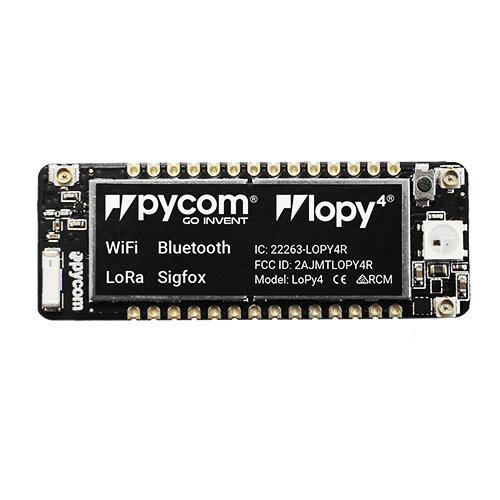
\includegraphics[keepaspectratio=true,scale=1.7]{pycom_lopy4.jpeg}
        \caption{pycom lopy 4}
  \end{minipage}
  \hfill
  \begin{minipage}[b]{0.4\textwidth}
   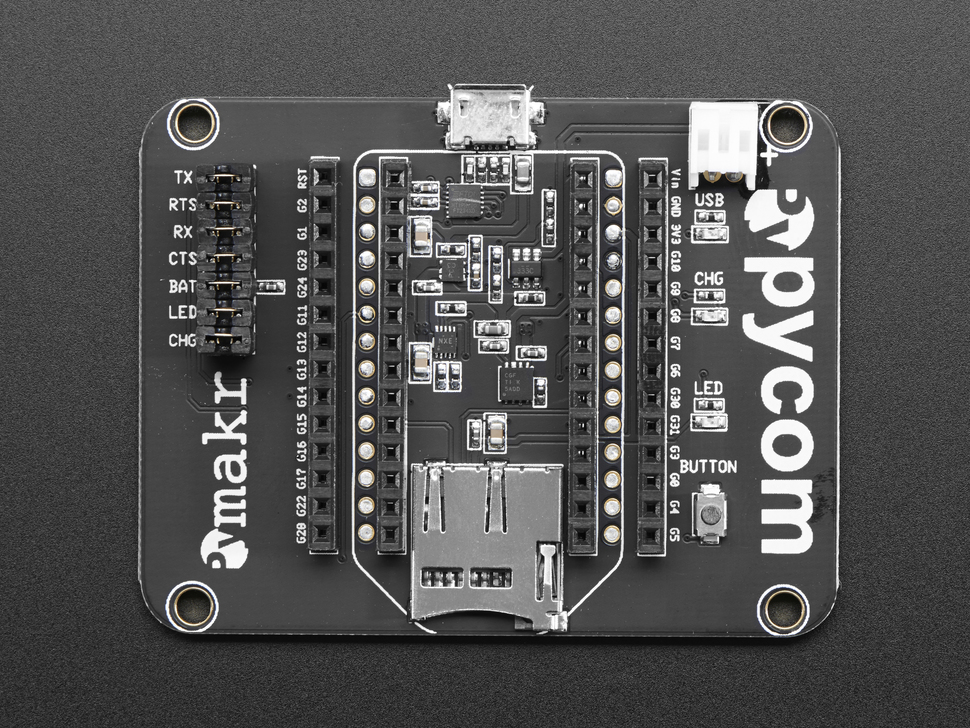
\includegraphics[keepaspectratio=true,scale=0.5]{pycom_expansion_board.jpeg}
    \caption{expansion board v3.0}
  \end{minipage}
\end{figure}

    \begin{figure}[H]
\begin{center}
\advance\leftskip-3cm
\advance\rightskip-3cm
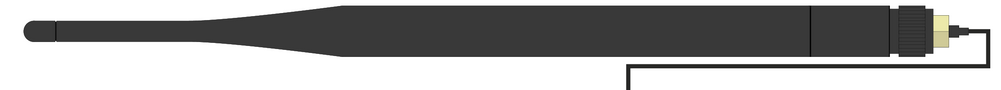
\includegraphics[keepaspectratio=true,scale=0.2]{lora_antenna.png}
\caption{antenne LoRa}
\label{visina8}
\end{center}\end{figure}



\section{Matériel}
\textcolor{red}{Branchez l'antenne LoRa avant d'alimenter la carte sinon la carte grille}\\
%Pour le branchement de l'antenne voir : \url{https://docs.pycom.io/gettingstarted/connection/lopy/}\\
%Pour le pinout des cartes d'extension voir : \url{https://docs.pycom.io/datasheets/boards/expansion3/},
%\url{https://docs.pycom.io/datasheets/boards/pytrack/}

\section{Démarrer la nanogateway}
\subsection{Code}

Clonez le dépôt : \url{https://github.com/CampusIoT/code-examples/tree/master/nanogateway_lopy}\\
Il contient 3 fichiers :
\begin{itemize}
    \item main.py
    \item config.py
    \item nanogateway.py
\end{itemize}\\

%Modifiez  config.py en renseignant le mot de passe wifi et son identifiant. \\

Informations complémentaires : \url{https://docs.pycom.io/tutorials/lora/lorawan-nano-gateway/} 

\subsection{Remplir le fichier config.py}

Dans config.py renseigner les champs WIFI\_SSID, WIFI\_PASS

\subsubsection{Obtenir le SSID du réseau WiFi}
\begin{minted}{bash}

iwgetid -r


\end{minted}

\subsection{Installer ATOM et pymakr}


\begin{comment}
\begin{minted}{bash}

wget -qO - https://packagecloud.io/AtomEditor/atom/gpgkey | sudo apt-key add -
sudo sh -c 'echo "deb [arch=amd64] https://packagecloud.io/AtomEditor/atom/any/ any main" 
> /etc/apt/sources.list.d/atom.list'
sudo apt-get update
sudo apt-get install atom


\end{minted}
atom pour lancer l'éditeur
\end{comment}
Télécharger la version 1.39.0 sur \url{https://github.com/atom/atom/releases/tag/v1.39.0}
Téléchargez le .deb. \\


informations complémentaires à : \url{https://flight-manual.atom.io/getting-started/sections/installing-atom/#platform-linux}

\subsubsection{installer pymakr}


Depuis atom selon l'image installer pymakr


    \begin{figure}[H]
\begin{center}
\advance\leftskip-3cm
\advance\rightskip-3cm
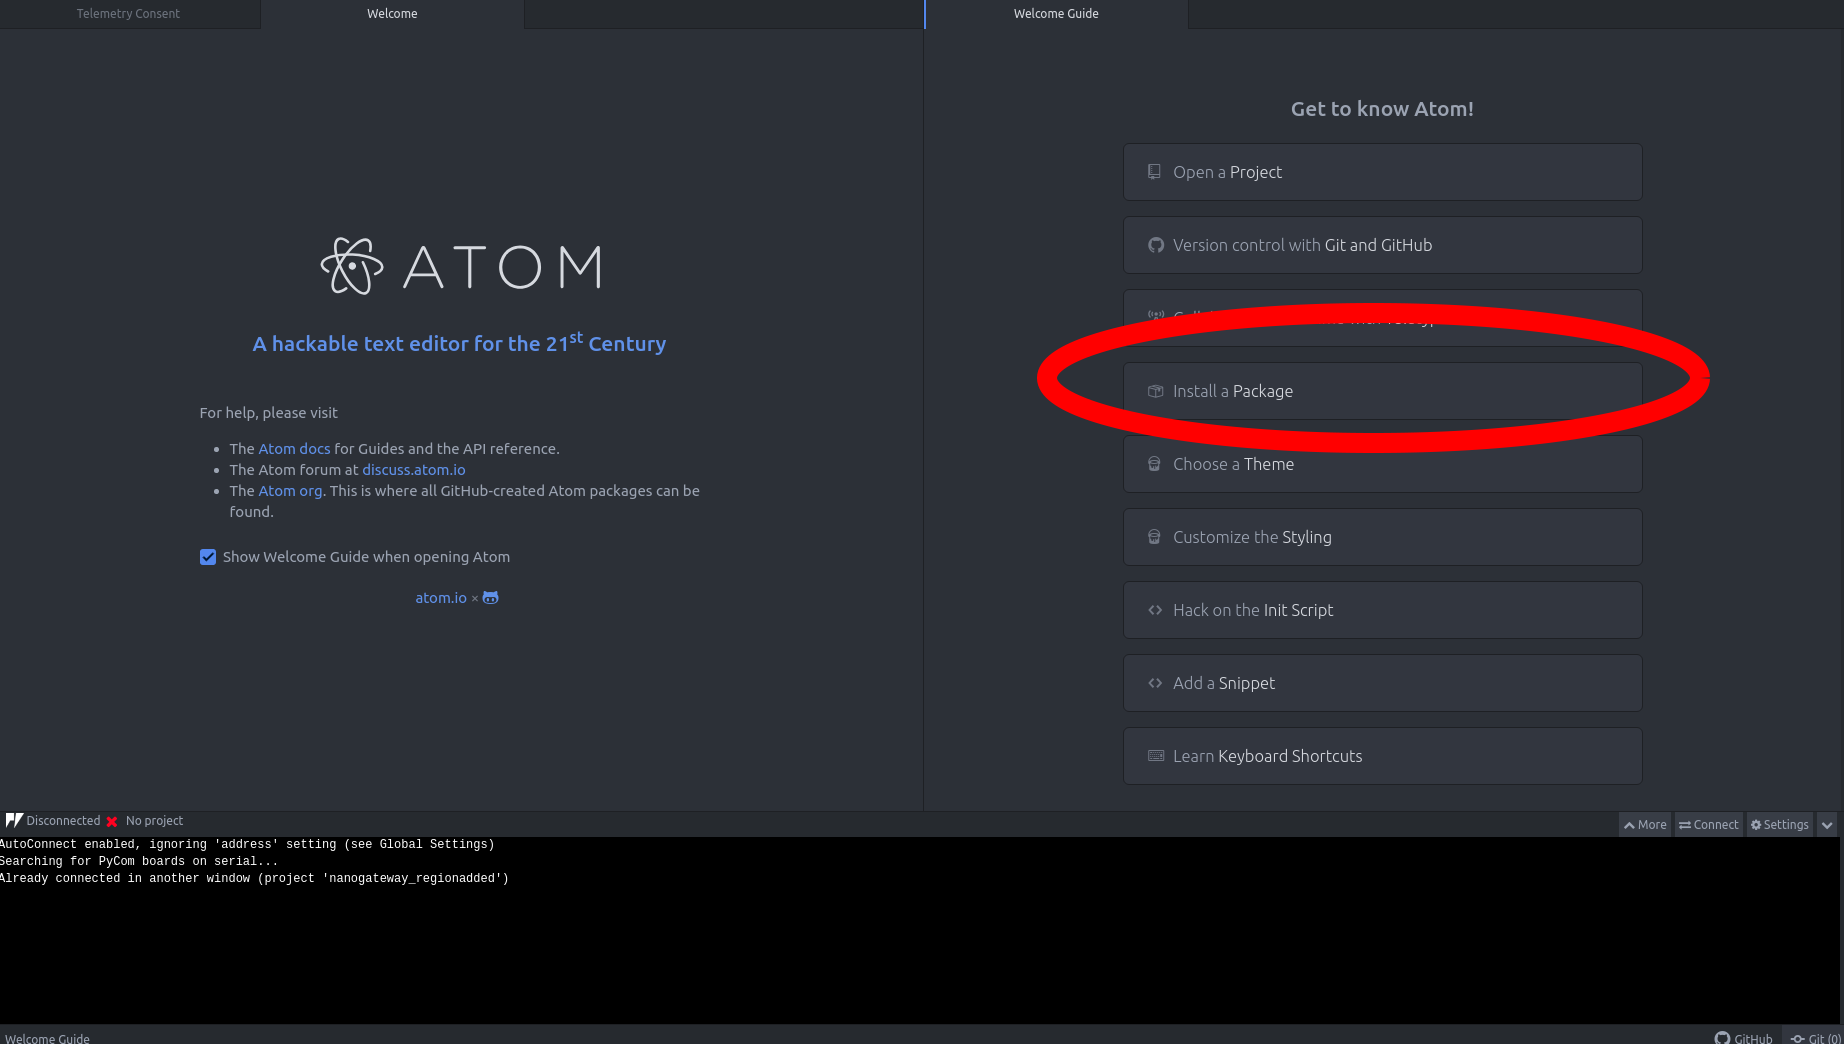
\includegraphics[keepaspectratio=true,scale=0.2]{atom_installpymakr.png}
\label{visina8}
\end{center}\end{figure}

Si il est impossible d'installer pymakr, installez une version antérieure à : \url{https://github.com/atom/atom/releases}\\
Désinstallez l'ancienne version :
\begin{minted}{bash}

sudo apt-get remove atom




\end{minted}

Pour ubuntu téléchargez le fichier .deb

Une alternative est aussi \textbf{Visual Studio Code}. \\

Informations complémentaires à  : \url{https://docs.pycom.io/pymakr/installation/atom/}

\subsection{Déverouiller les ports USB}
\subsubsection{Solution temporaire} 


\begin{minted}{bash}
sudo chmod 666 /dev/ttyACM0
\end{minted}
Il faut entrer cette commande souvent. \\
\subsubsection{Solution permanente}\\

Créer un fichier dans son home

\begin{minted}{bash}
50-myusb.rules
\end{minted} 

l'éditer : 

\begin{minted}{bash}
KERNEL=="ttyACM[0-9]*",MODE="0666"
\end{minted}

Puis copier ce fichier dans /etc/udev/rules.d/ et redémarrer votre PC.

\begin{minted}{bash}
 sudo cp 50-myusb.rules /etc/udev/rules.d
\end{minted}
C'est suffisant pour ne plus avoir à réouvrir les ports manuellement. Cependant, n'importe quel dispositif usb connecté au PC a maintenant le droit d'écriture sur le PC. \\

Pour plus de sécurité ajouter ces lignes dans ce fichier :

\begin{minted}{bash}
ACTION=="add", KERNEL=="ttyACM[0-9]*", ATTRS{idVendor}=="xxxx", 
ATTRS{idProduct}=="yyyy", MODE="0666"
\end{minted}
 
 Pour déterminer idVendor et idProduct des cartes tapez lsusb avant et après avoir connecté la carte. \\

 Dans mon cas :
 
 \begin{figure}[H]
\begin{center}
\advance\leftskip-3cm
\advance\rightskip-3cm
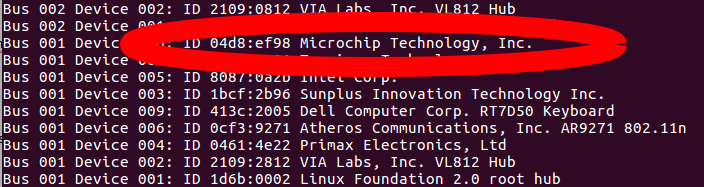
\includegraphics[keepaspectratio=true,scale=0.5]{lsusb.png}
\label{visina8}
\end{center}\end{figure}

idProduct = ef98\\
idVendor= 04d8\\




\subsection{Démarrer la nanogateway}

\subsubsection{Télécharger le code sur la carte}
Selon l'image utiliser la console d'Atom pour se connecter à la carte :
Si la carte ne se connecte pas, appuyer sur le boutuon reset.


  \begin{figure}[H]
\begin{center}
\advance\leftskip-3cm
\advance\rightskip-3cm
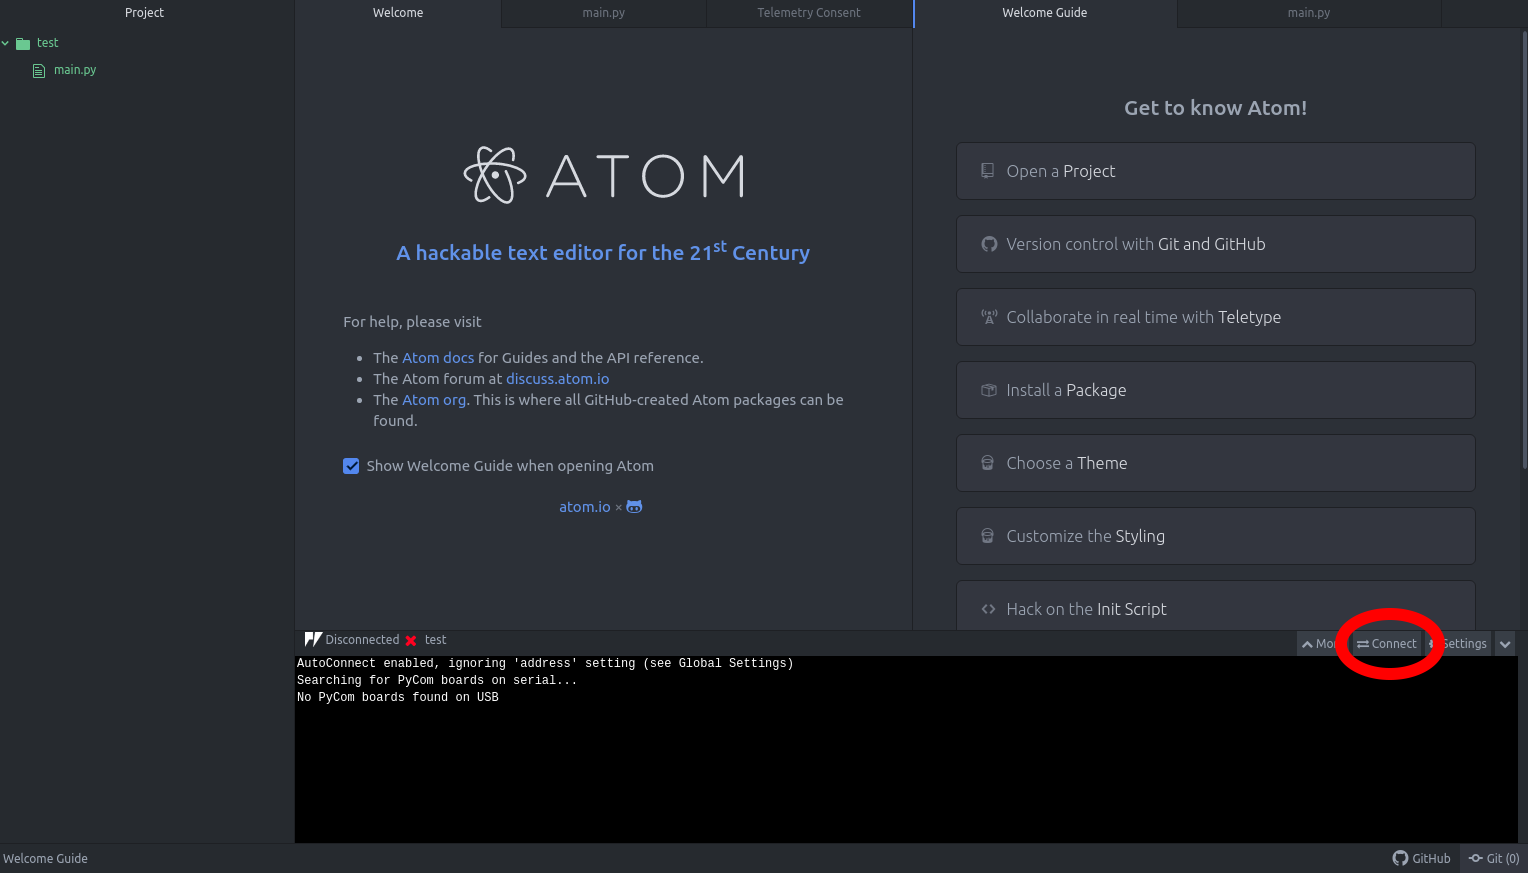
\includegraphics[keepaspectratio=true,scale=0.3]{atom_connect.png}
\label{visina8}
\end{center}\end{figure}

Dans Atom File, Open Folder pour choisir son projet puis cliquer sur Upload dans la console Pymakr pour télécharger le  code sur la carte.

\begin{figure}[H]
\begin{center}
\advance\leftskip-3cm
\advance\rightskip-3cm
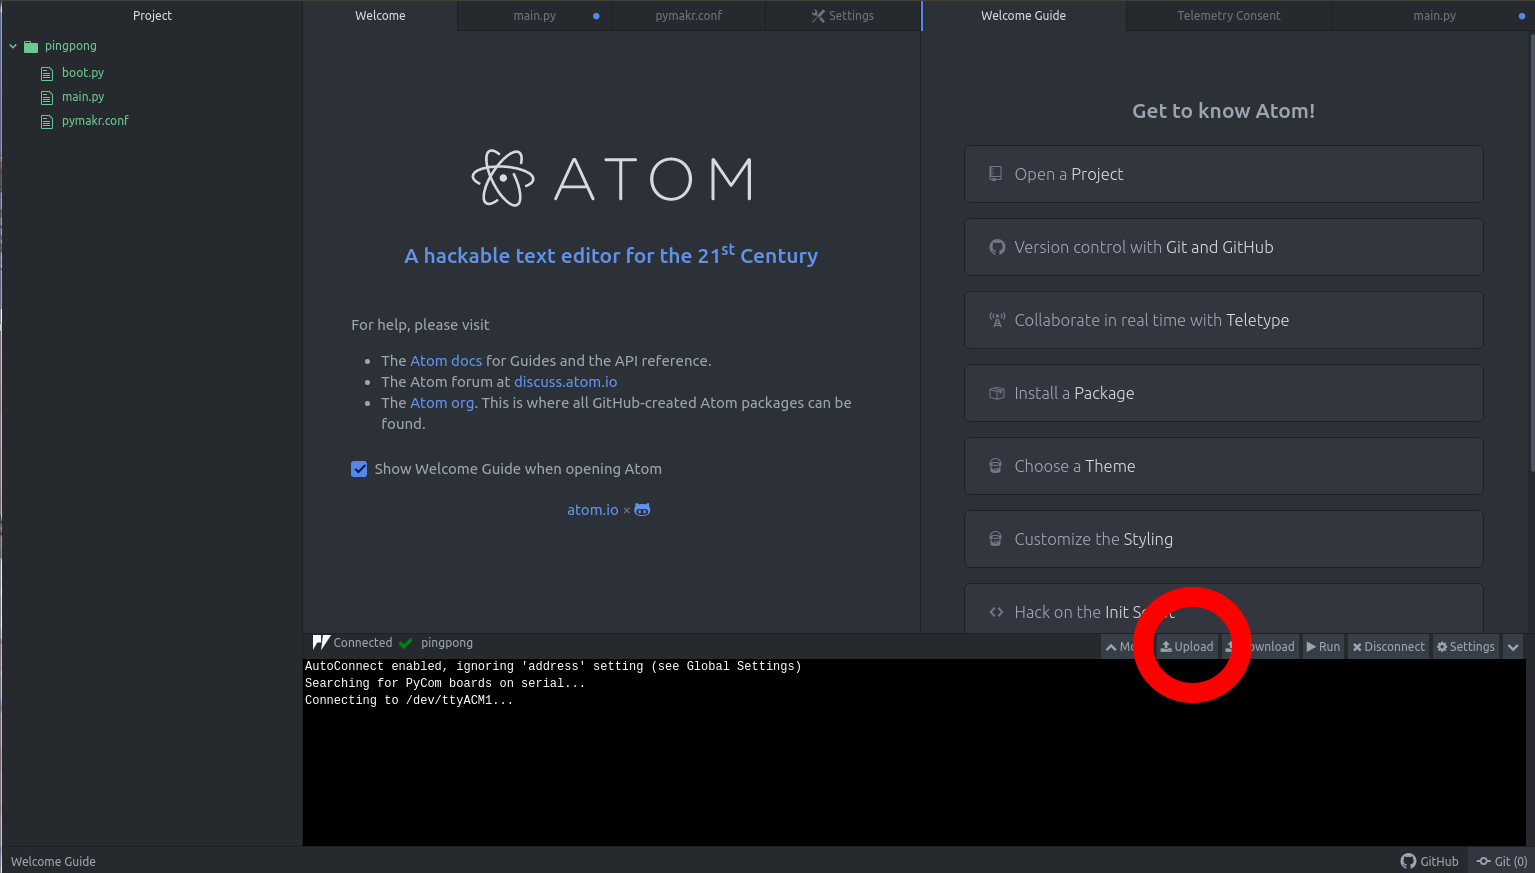
\includegraphics[keepaspectratio=true,scale=0.3]{atom_upload.png}
\label{visina8}
\end{center}\end{figure}

Le texte suivant doit s'afficher :

\begin{figure}[H]
\begin{center}
\advance\leftskip-3cm
\advance\rightskip-3cm
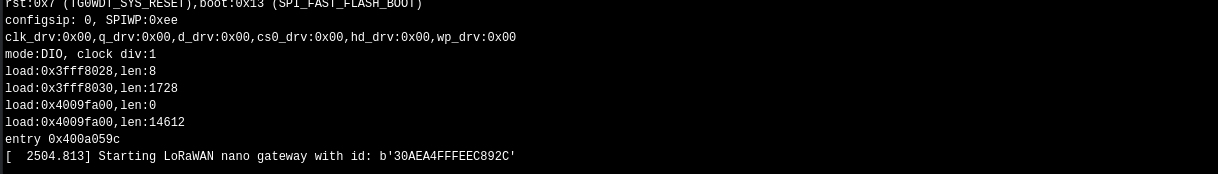
\includegraphics[keepaspectratio=true,scale=0.5]{nanogateway_lopy.png}
\label{visina8}
\end{center}\end{figure}

%\section{Connecter la gateway à LoRaWAN }

Patienter après que le prompt mycropython s'affiche selon l'image.

Une fois la connexion avec le serveur établie les messages suivants s'affichent :

\begin{figure}[H]
\begin{center}
\advance\leftskip-3cm
\advance\rightskip-3cm
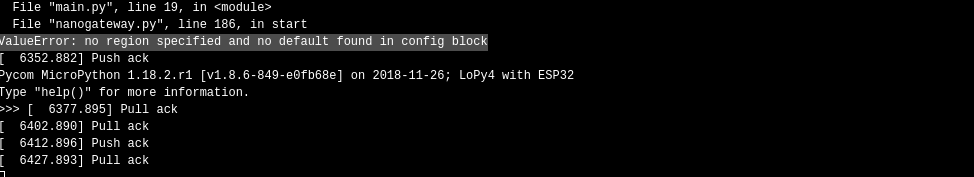
\includegraphics[keepaspectratio=true,scale=0.6]{nano_gateway2.png}
\label{visina8}
\end{center}\end{figure}


\section{Enregistrer la nanogateway sur The Things Network}

\subsection{Se créer un compte sur The Things Network}

\url{https://www.thethingsnetwork.org/}

\section{Enregistrer la gateway}


\begin{figure}[H]
\begin{center}
\advance\leftskip-3cm
\advance\rightskip-3cm
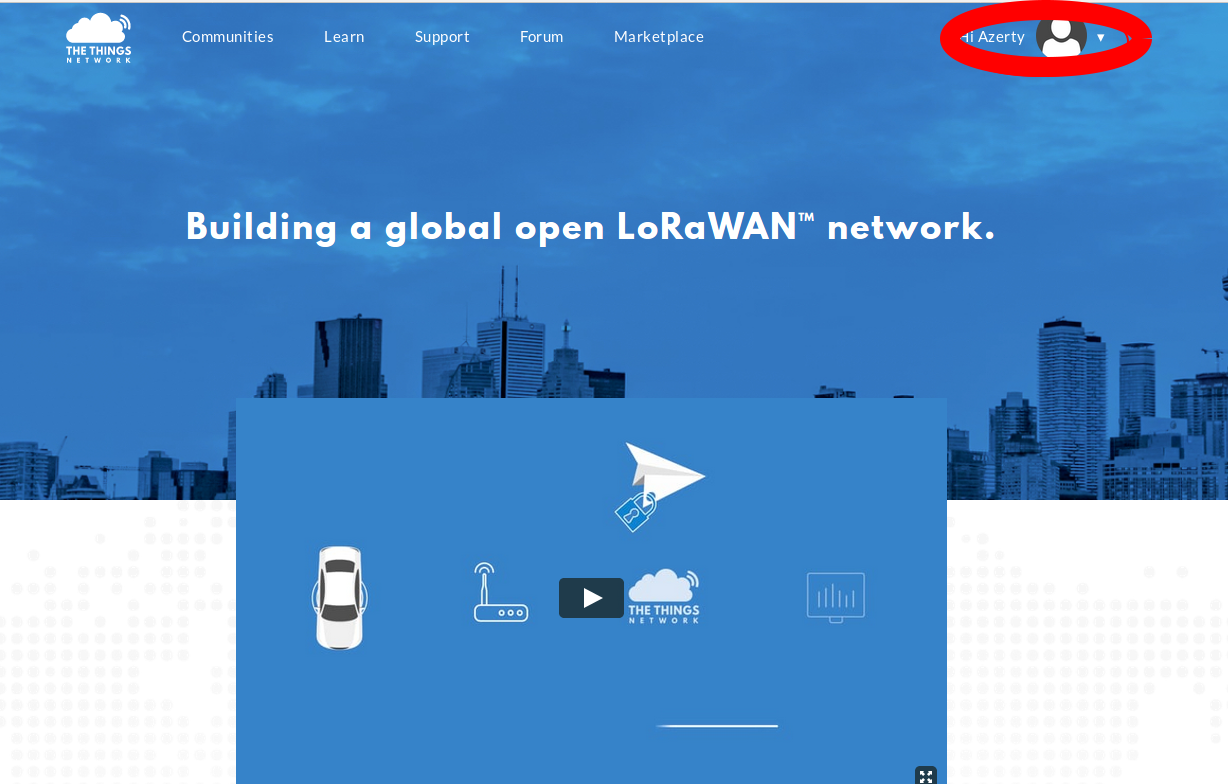
\includegraphics[keepaspectratio=true,scale=0.2]{ttn_console.png}
\label{visina8}
\end{center}\end{figure}

Cliquer sur l'icône selon l'image puis cliquer sur Console.
Ensuite choisir Gateways, puis register gateway.



\begin{figure}[H]
\begin{center}
\advance\leftskip-3cm
\advance\rightskip-3cm
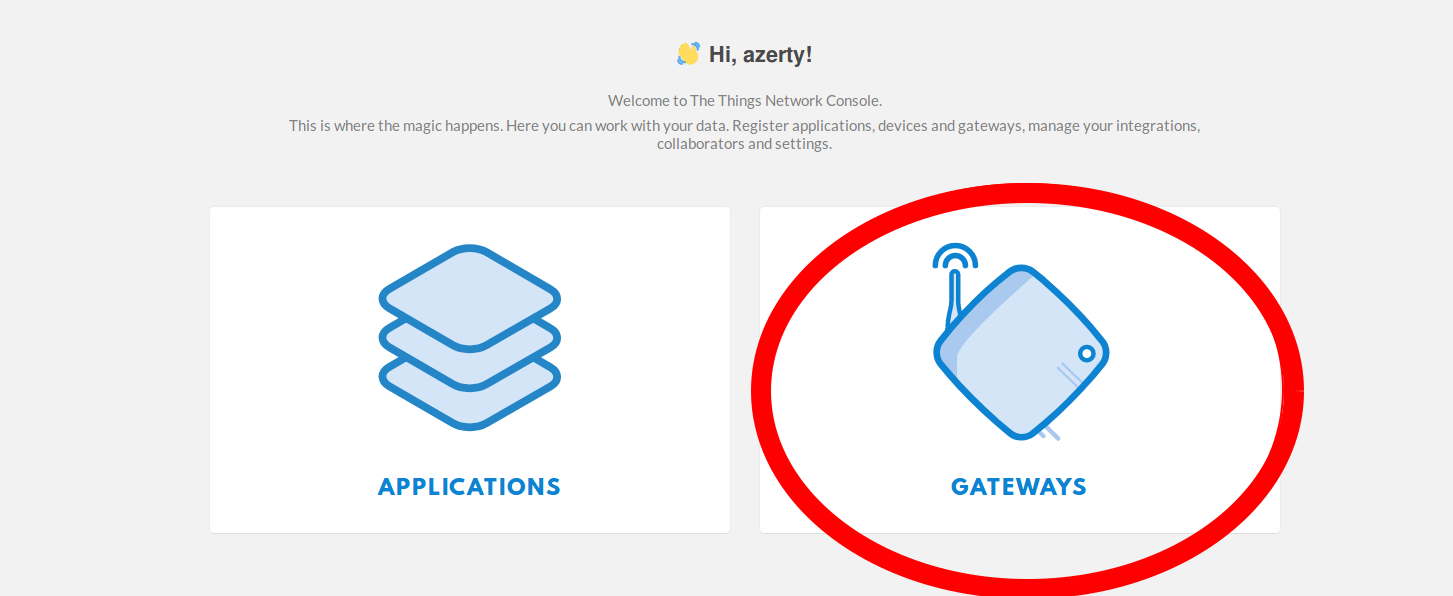
\includegraphics[keepaspectratio=true,scale=0.2]{ttn_registergateway.png}
\label{visina8}
\end{center}\end{figure}

Cochez \textit{legacy packet forwarder} comme sur l'image :


\begin{figure}[H]
\begin{center}
\advance\leftskip-3cm
\advance\rightskip-3cm
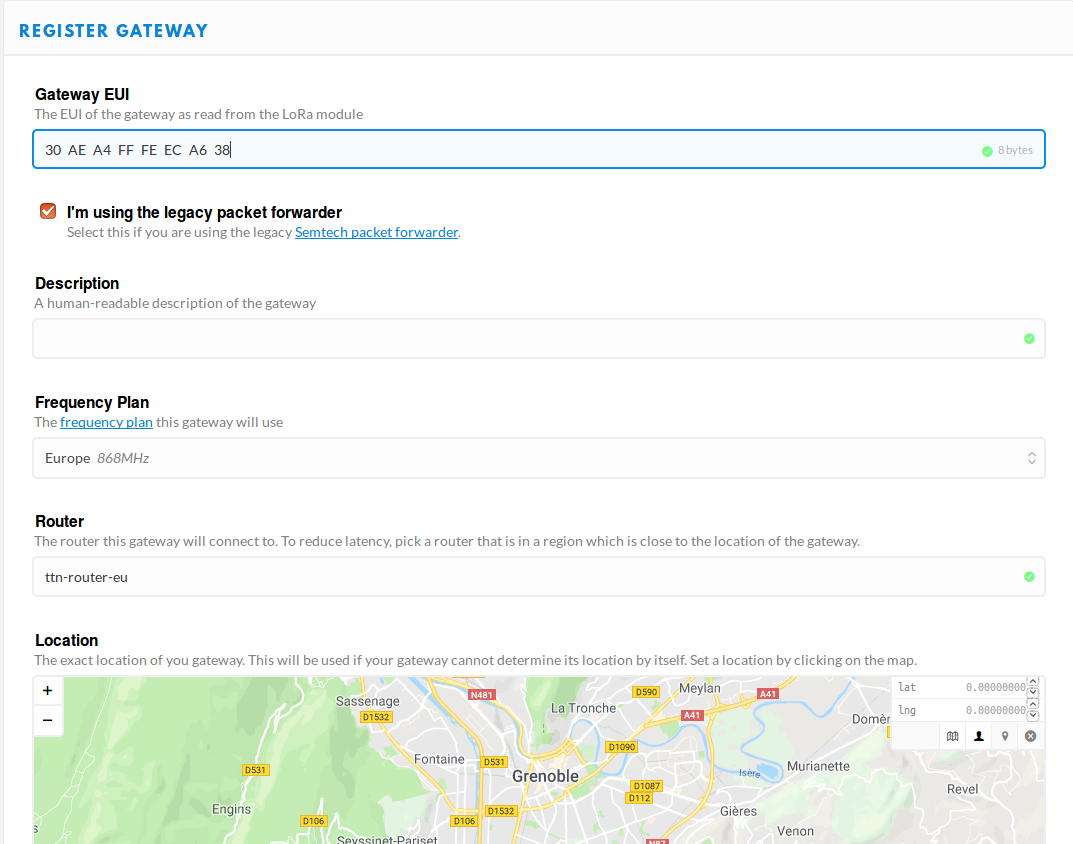
\includegraphics[keepaspectratio=true,scale=0.3]{register_gateway.png}
\label{visina8}
\end{center}\end{figure}


\subsection{Remplir le champ Gateway EUI}




\subsubsection{Méthode 1}
Au démarrage de la nanogateway :
 \begin{figure}[H]
\begin{center}
\advance\leftskip-3cm
\advance\rightskip-3cm
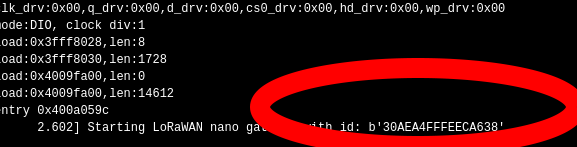
\includegraphics[keepaspectratio=true,scale=0.4]{gateway_id_atom.png}
\caption{antenne LoRa}
\label{visina8}
\end{center}\end{figure}
 
 
 \subsubsection{Méthode 2}
Le Gateway ID est de la forme XX XX XX F FFE XX XX XX \\
Où XX XX XX XX XX est la valeur retournée par la fonction \textit{machine.unique\_id()}.\\


\begin{comment}
Avec ifconfig : 
\begin{figure}[H]
\begin{center}
\advance\leftskip-3cm
\advance\rightskip-3cm
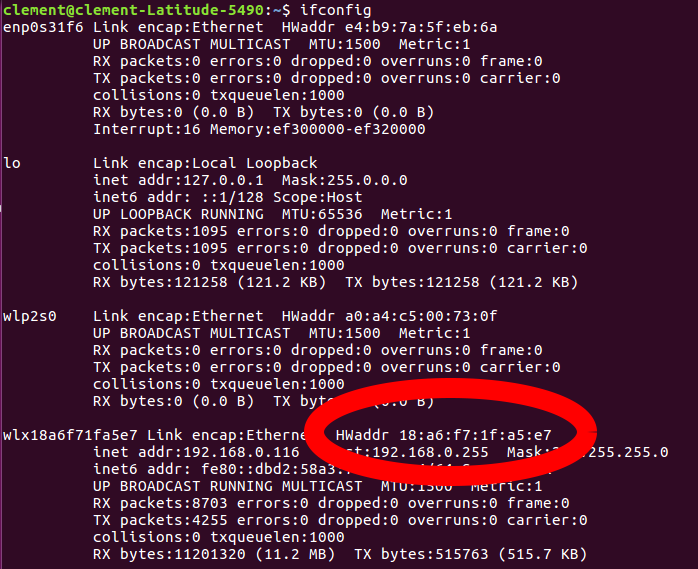
\includegraphics[keepaspectratio=true,scale=0.4]{ifconfig.png}
\caption{antenne LoRa}
\label{visina8}
\end{center}\end{figure}

Dans mon cas cette adresse est 18 a6 f7 1f a5 e7
\end{comment}

Créer un dossier contenant un fichier main.py :
\begin{minted}{python}

import machine
import ubinascii

WIFI_MAC = ubinascii.hexlify(machine.unique_id()).upper()
print(WIFI_MAC)



\end{minted}

Télécharger le code sur la carte et l'ID s'affichera dans la console d'Atom.\\

informations complémentaires à \url{ https://docs.pycom.io/tutorials/lora/lorawan-nano-gateway/}\\\\

Le statut de la gateway est maintenant \textit{connected}

\begin{figure}[H]
\begin{center}
\advance\leftskip-3cm
\advance\rightskip-3cm
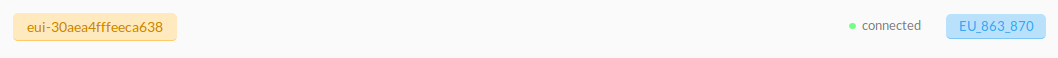
\includegraphics[keepaspectratio=true,scale=0.4]{gateway_connected.png}
\label{visina8}
\end{center}\end{figure}



\end{document}
